\section{Methodology}

\subsection{Description of the data}
For classifying fake news, Wang's Liar dataset will be used \cite{wang2018}. 
The Liar dataset contains 12.791 short statements from Politifact.com, which are labeled manually by a Politifact.com editor on truthfulness.
The speakers in the dataset include both representatives from the two major political parties in the United States, as well as a large amount of social media posts. 

The statements are an average of 18 tokens long, and the topics vary from different political subjects, as can be seen in figure 1.
Truthfulness is evaluated by assigning one of 6 labels, ranging from \textit{pants-on-fire} to \textit{true}. 
The distribution of statements across the 6 labels can be seen in table 2.

\begin{figure}[h]
    \centering
    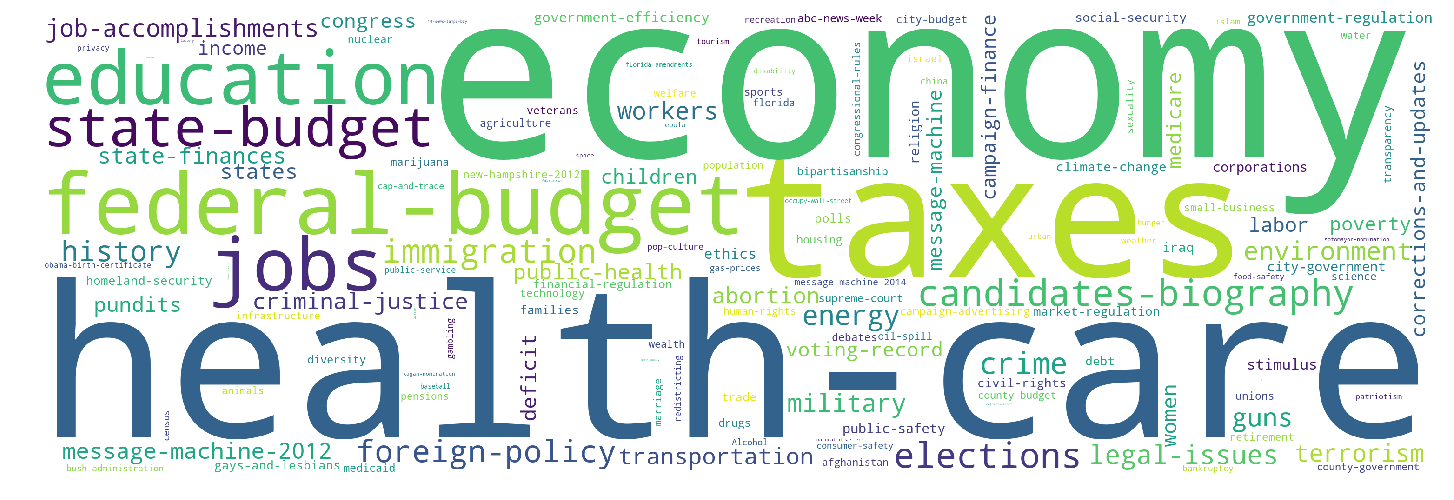
\includegraphics[width=0.9\columnwidth]{subjectwordcloud}
    \caption{An overview of all statement topics in the Liar dataset.}
\end{figure}

For each statement, the dataset contains an id, a label, a subject, a speaker, the function title of the speaker, the affiliated state and political affiliation, the context of the statement and a vector with a truthfulness history.
An example of such a data entry can be seen in table 1.
Wang introduced this truthfulness history to boost the prediction scores, as speakers with a track record of lying are expected to have a lower chance of speaking the truth when classifying new statements.
However, for our application we are only interested in the statement itself and its corresponding label. 
Due to cheapness and spreadability, a large amount of fake news is spread over social media \cite{shu2017}. 
This means author information and metadata will not readily be available in real world circumstances.

\begin{table*}[t]
    \centering
    \begin{tabular}{ll}
        \hline
        id                     & 11044.json                                                      \\ \hline
        label                  & pants-fire                                                      \\ \hline
        statement              & The Mexican government forces many bad people into our country. \\ \hline
        subjects               & foreign-policy,immigration                                      \\ \hline
        speaker                & donald-trump                                                    \\ \hline
        speaker\_job           & President-Elect                                                 \\ \hline
        state                  & New York                                                        \\ \hline
        party                  & republican                                                      \\ \hline
        context                & an interview with NBC's Katy Tur                                \\ \hline
        mostly\_true\_count    & 37                                                              \\ \hline
        half\_true\_count      & 51                                                              \\ \hline
        barely\_true\_count    & 63                                                              \\ \hline
        false\_count           & 114                                                             \\ \hline
        pants\_on\_fire\_count & 61                                                              \\ \hline
    \end{tabular}
    \caption{An example entry in the Liar dataset.}
\end{table*}

The original dataset has been split beforehand into a test, train and validation set. 
The train set contains 80\% of the total amount of statements, while the test and validation set both contain approximately 10\% of the statements. 

\subsection{Data preprocessing and cleaning}
\subsubsection{Filtering statements}
The original dataset contained statements ranging from 1 sentence to 19. 
On closer inspection of statements with the high amounts of sentences, it was found that not all statements were processed from source files into dataframes correctly.
As a result, records of some different statements were joined together, forming a single string.
To combat this, the following regular expression was used to filter those statements out:\\

\begin{quote}
    \begin{scriptsize}
        \begin{verbatim}
            \.json\t(mostly-true|true|half-true|false|barely-true|pants-fire)
        \end{verbatim}
    \end{scriptsize}
\end{quote}

After applying this regular expression, the total amount of sentences in the statements were reduced from a maximum of 19 to a maximum of 11. 
This reduced the original reported size of the dataset by 52 statements to a total of 12784. 

\subsubsection{Reducing labels}

Wang's main objective was to classify fake news into a fine-grained category of fakeness \cite{wang2018}.
For our main research question, we aim to predict whether the statements are fake news or not. 
This means the statements do not necessarily need to be distinguished into these fine-grained categories.
Because of this, the classifiers used to predict fake news in this research will be trained on Khurana's division into 3 labels instead of the original 6 \cite{khurana2017}.
The division from the original 6 labels into the 3 labels can be seen in table 2. 
This way, we can compare performance of pre-trained embeddings to Khurana's purely traditional, linguistic approach to classification of this dataset.

\begin{table}[]
    \centering
    \begin{tabular}{|l|l|}
        \hline
        \textbf{6 labels}                                              & \textbf{3 labels}                                                          \\ \hline
        \begin{tabular}[c]{@{}l@{}}true\\ (16.1\%)\end{tabular}        & \multirow{2}{*}{\begin{tabular}[c]{@{}l@{}}true\\ (35,3\%)\end{tabular}}   \\ \cline{1-1}
        \begin{tabular}[c]{@{}l@{}}mostly-true\\ (19.2\%)\end{tabular} &                                                                            \\ \cline{1-2}
        \begin{tabular}[c]{@{}l@{}}half-true\\ (20.5\%)\end{tabular}   & \begin{tabular}[c]{@{}l@{}}half-true\\ (20.5\%)\end{tabular}               \\ \hline
        \begin{tabular}[c]{@{}l@{}}barely-true\\ (16.4\%)\end{tabular} & \multirow{3}{*}{\begin{tabular}[c]{@{}l@{}}false\\ (44,19\%)\end{tabular}} \\ \cline{1-1}
        \begin{tabular}[c]{@{}l@{}}false\\ (19.6\%)\end{tabular}       &                                                                            \\ \cline{1-1}
        \begin{tabular}[c]{@{}l@{}}pants-fire\\ (8.19\%)\end{tabular}  &                                                                            \\ \hline
    \end{tabular}
    \caption{Distribution of labels from the original label distribution when reducing the amount of labels.}
\end{table}

\subsection{Methods}

\subsubsection{Applying embedding techniques}
As our main research question is focussed on pre-trained word embeddings, the first step in the classification process is to turn the statements of the Liar dataset into vectors. 
For this purpose, the Flair framework will be used. 
Flair contains interfaces for turning words into embeddings, built on the PyTorch platform \cite{flairrepo}\cite{pytorch}. 
Using Flair, we have access to the following 5 state-of-the-art pre-trained embedding techniques: 
\begin{itemize}
    \item ELMo (Embeddings from Language Models) \cite{peters2018};
    \item BERT \cite{devlin2018};
    \item Generative Pre-Training (GPT) \cite{radford2018};
    \item Transformer-XL \cite{dai2019};
    \item Flair \cite{akbik2019};
    \item GPT-2 \cite{radford2019}.
\end{itemize}

For each of our embedding techniques, we will generate a new dataset with statements from the Liar dataset in their embedded form. 
These datasets will then be used for classification, without the datasets being specifically adjusted or finetuned for specific models.
This allows us to independently compare classification models for each of our embedding techniques. 

To apply these embeddings, the Flair framework first requires a sentence object to be created \cite{flairsentence}.
For dividing the statements into sentences, the \texttt{sent\_tokenize} function from the \texttt{nltk} package will be used \cite{nltktokenize}. 
After applying this split, Flair's sentence object takes care of tokenization and applying the selected embedding technique.
This way, all statements of the Liar dataset will be turned into other representations one by one and saved for future use.

\paragraph{Embeddings from Language Models (ELMo)}
The first word embedding technique, ELMo, is based on a bidirectional language model. 
ELMo embeddings are different from regular word embeddings, because each token is a function of the entire input sentence.
The underlying neural network architecture consists of a bidirectional LSTM trained on a large corpus.
This corpus contained approximately 5.5 billion tokens, crawled from Wikipedia and WMT 2008-2012.

The representation is formed from combining internal states of the LSTM. 
The higher level LSTM states capture context-dependent aspects of word meaning, while the lower level states model aspect of syntax.
Combining these internal states allows for rich representations that capture both complex characteristics of word use (syntax and semantics) and how word uses vary across linguistic contexts \cite{peters2018}.

The model for our use will be the original ELMo model, containing 93.6 million parameters.
Each created word vector has a length of 3072. 

\paragraph{Generative Pre-Training (GPT)}
OpenAI's GPT model is among the first text embedding methods to use the Transformer architecture by Vaswani et al. \cite{vaswani2017}, as described in section 2.2.
Radford et al. chose specifically for this architecture, as these types of models allow for a more structured memory for handling long-term dependencies in text.
This results in a robust transfer performance across different tasks. 

GPT's training procedure consists of two stages: learning a language model on a large corpus of text, and a fine-tuning stage, where the model is adapted to a task with labeled data.
For learning the language model, the BooksCorpus dataset was used, which contains over 7000 books, and is of comparable size to the datasets used to pre-train ELMo embeddings \cite{radford2018}.

Each created word vector has a length of 1536.

\paragraph{Flair}
Just like the ELMo embeddings proposed by Peters et al. \cite{peters2018}, Akbik et al. proposed Flair embeddings, which are contextualized word embeddings on a character level.
According to these authors, \textit{contextual string embeddings are powerful embeddings that capture latent syntactic-semantic information that goes beyond standard word embeddings. 
Key differences are: (1) they are trained without any explicit notion of words and thus fundamentally model words as sequences of characters. 
And (2) they are contextualized by their surrounding text, meaning that the same word will have different embeddings depending on its contextual use} \cite{flairembedding}. 

Flair embeddings make use of a bidirectional LSTM architecture for language modelling. 
For pre-training, a sequence of characters is passed to this architecture, which at each point in the sequence is trained to predict the next character.
Then, the hidden states of the neural network are used to create contextualized word embeddings.

Akbik et al. also proposed the concept of stacking embeddings, allowing for traditional word embeddings to be combined with Flair embeddings.
This has the potential to create word vectors that contain greater latent word-level semantics by concatenating embedding vectors trained on a character level and on a word level \cite{akbik2018}.

For our use, the recommended configuration of stacked embeddings by the Flair repository are used \cite{flairembedding}: this is a combination of GloVe word embeddings \cite{pennington2014} and both forward and backward Flair embeddings.
Each created word vector from these stacked embeddings has a length of 4196, which is the longest vector length of all embedding techniques listed in section 3.3.1. 

\paragraph{Bidirectional Encoder Representations from Transformer (BERT)}
Devlin et al. propose an embedding technique which is also based on the Transformer architecture described in section 2.2, but differs from the GPT Transformer, as it is trained using bi-directional self-attention instead of GPT's constrained left-only self-attention.
Pre-training is conducted on 2 unsupervised learning tasks. 
The first utilizes a masked language model (MLM), which randomly masks some of the tokens from the input with the objective to predict the masked word, based only on its context.
This MLM fuses the context to the left and to the right, allowing pre-training of a deep bi-directional Transformer architecture.
In the second task, the model takes a sentence, and predicts the next sentence in the sequence. 
The first task is aimed on word level, while this second learning task aims at the model's sentence level understanding \cite{devlin2018}. 

The model used for embedding our statements will be the original BERT Uncased model, which contains 110 million parameters and 12 layers. 
Pre-training for this model was conducted using a combination of the BooksCorpus (800 million words) and Wikipedia (2500 million words).
Each created word vector has a length of 3072. 

\paragraph{Transformer-XL}
Dai et al. build further on the original Transformer architecture with the Transformer-XL model, but add recurrence to allow for the model to conserve hidden states across batches.
This means that for each new batch, the model uses previous batches to predict the first few symbols of the current batch.
By using this concept of recurrence, the Transformer-XL architecture allows for creating long-term dependencies \cite{dai2019}. 

The model is pre-trained on the WikiText-103 dataset, which contains over 100 million tokens and is particularly focussed on long-term dependencies \cite{merity2017}. 
Each created word vector has a length of 1024. 

\paragraph{GPT-2}


\subsubsection{Pooling and padding}
For our classification tasks, we need to transform the shape of our data to a uniform style.
As described in section 2.3 and 2.4, we will make use of pooling and padding techniques to achieve this.

\paragraph{Applying pooling}
In section 2.3, we have identified three simple mathematical operations to reduce our vector length to a fixed length.
We will apply average pooling, max pooling and min pooling and test their accuracies on a classifier to test what pooling technique works best for each embedding technique.
For applying these transformations, the NumPy package will be used \cite{numpy}.
NumPy contains tools for working with multi-dimensional arrays, and allows us to easily manipulate data. 

\begin{figure}[h]
    \centering
    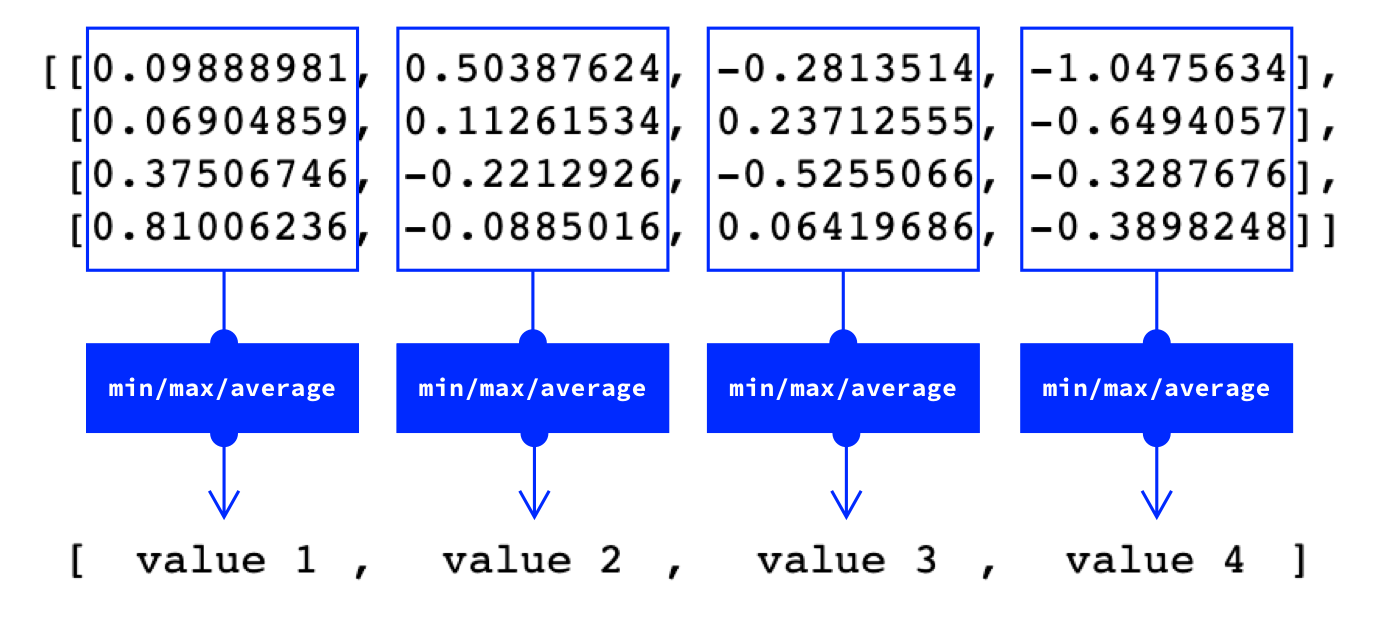
\includegraphics[width=0.9\columnwidth]{applyingpooling}
    \caption{Applying pooling to reduce a matrix to a single vector.}
\end{figure}

As can be seen in figure 2, applying a pooling operation is rather straight-forward: for every word vector, the floating point number at every $n$th index is gathered.
After that, a mathematical operation is performed to reduce those numbers to a single number, which will become the number in the $n$th index of the final full statement vector.

\paragraph{Applying padding}
For neural architectures, three-dimensionally shaped data can be used for classification. 
However, the problem still remains that each text sequence can have a different length of words. 
Padding the sequences, as described in section 2.4, will be used to combat this.

For applying padding, we will use the \texttt{pad\_sequences} function from the Keras library \cite{keraspad}. 
This function allows us to specify a maximum sequence length to transform all our statements into.

\paragraph{doc2vec}
Of course, both pooling and padding result in some loss of data.
To compare these data densing techniques to a situation in which all words of full sequences are taken into account, results using a doc2vec embedding will also be taken into account.
The doc2vec model creates paragraph vectors instead of word vectors, allowing all text in each statement to condense back into one single vector, without specifiying a cut off point or a maximum length \cite{le2014}.

Together with the majority vote and the best score from previous research, the doc2vec score will function as a baseline for comparing performance of our classifiers.
For gathering doc2vec scores, the doc2vec interface in the Gensim library will be used \cite{gensim}. 

\subsubsection{Classification}
To make the results of our embedding techniques comparable to existing research, four classifiers of Wang and the top performing model of Khurana will be used to classify our statements \cite{wang2018}\cite{khurana2017}:

\begin{enumerate}
    \item Logistic regression;
    \item SVM;
    \item Gradient Boosting;
    \item Bidirectional LSTM;
    \item Convolutional neural network.
\end{enumerate}

For all classifiers, hyperparameters will be tuned on the validation set to keep the experimental settings as close to the original setup by Wang as possible.
Performance of the classifications will be reported using accuracy over the test set as an evaluation metric, similar to the research conducted by Khurana and Wang \cite{wang2018}\cite{khurana2017}. 
To reduce as much random effects as possible on the neural classifications, each neural classification will be run 5 times, and the reported score will be the average of those 5 scores. 

For the first three non-neural classification algorithms, scikit-learn will be used for implementation \cite{scikit-learn}. 
To tune the regularization strength for the logistic regression and SVM implementation and to tune the learning rate of the gradient boosting, a grid search will be used. 

The Keras library will be used for the neural architectures \cite{keras}.
Both neural classifiers will use a dropout keep probability of 0.8.
A batch size of 32 and 5 training epochs will be set. 
The convolutional neural network will consist of three layers with a filter size of (2, 3, 4).
Each layer will implement 128 filters and will utilize a ReLu activation function.